\documentclass{article}
\usepackage[UTF8,scheme=plain,fontset=fandol]{ctex}
\usepackage[preprint]{corl_2026}
\setmainfont{TeX Gyre Termes}
\usepackage{amsmath,amssymb,booktabs,graphicx}
\hypersetup{pdftitle={面向延迟感知的非生成式机器人判断：配对仿真研究},pdfsubject={中文内部研究稿，未投稿},pdfauthor={}}
\title{面向延迟感知的非生成式机器人判断：\\一项可复现的配对仿真研究}
\author{中文内部研究稿 · 2026 年 9 月 23 日\\作者与单位待研究团队确认}
\begin{document}
\maketitle
\begin{abstract}
机器人获取更精确的观测需要时间，而这段时间内的动作可能改变信息的价值。
我们研究一个受限但可审计的问题：在固定操作技能执行中，从继续执行、停住刷新、边动边刷新三个候选中选择延续方式。
我们构建共享的非生成式候选后果判断器，并在 MuJoCo Fetch 推物和抓取放置任务上，从完整相同物理状态分叉生成监督标签。
阶段判断实验包含 1,500 个检查点、4,500 次候选执行和 12 个训练模型，检查点与模型选择严格分离。
在长延迟抓取中，完整判断器三个种子的平均成功率为 97.4\%，固定异步刷新为 91.1\%；但同分布抓取的简单阶段查表优于完整模型，动作历史的独立收益没有得到支持。
另在 600 个全新场景上完成一轮等预算 RSI 数据更新检验，反例采样相对随机采样的成本差区间跨零。本文保留正负结果；当前证据不足以证明普遍算法优势或额外采样效率。
\end{abstract}
\keywords{机器人判断，延迟感知，配对仿真，主动感知，非生成式模型}

\section{引言}
机器人在动作执行中面对的不确定性，不仅来自观测内容，也来自观测在何时采集、何时返回，以及等待期间执行了什么动作。
即使较慢的感知方法能提供更精确的位置估计，机器人收到结果时，接触关系和物体位置也可能已经改变。
因此，将更高感知精度等同于更高任务成功率，或者用固定刷新周期覆盖所有操作阶段，都可能产生不必要的等待或错误动作。

本文受到结构化、非生成式判断接口的启发~\citep{jev2026}，将决策限定为固定候选的数值评估。
推理时无需 GPT 生成完整文字计划，也不生成新的低层轨迹：任务目标和低层技能预先给定，小网络只判断应该如何获取与消费证据。
这一限制允许我们控制技能、起点、可见信息和剩余时间预算，考察收益究竟来自信息决策还是低层控制差异。

本稿记录的实际贡献是一个可复现的物理实验协议、一组经过状态与回放核验的配对记录，以及针对阶段、观测年龄和动作历史的消融结果。
研究对象限定为结构化状态上的小型判断器，不代表官方 Jev 或视觉语言模型的能力。
阶段条件化、反事实标签或有限候选接口本身均已有广泛先例；论文方向能否成立，需要依靠同条件强基线与新分布验证。

\section{相关工作与研究边界}
\paragraph{主动感知与信息价值。}
Krishna 等研究机器人任务中感知信息的价值~\citep{krishna2025value}。
Hu 等提出 AAWR，在训练时利用额外特权传感器估计优势，学习现实机器人的主动感知行为~\citep{hu2025aawr}。
因此，“让机器人学会再看一次”并不是本研究的新颖性主张。
本文采用固定技能和有限候选，研究延迟下的信息消费方式；目前没有复现 AAWR，不能作性能优越性比较。

\paragraph{异步执行与时刻错位。}
REMAC 将执行失败的重要来源定位为动作块与当前感知的不一致，并通过 masked action chunking 学习修正~\citep{wang2026remac}。
FutureRTC 则预测执行时刻的观测和本体状态~\citep{jiang2026future}。
我们保留其所强调的时间错位问题，但当前学习对象是感知候选的结果价值，而非动作块或未来视觉表示。
判断器与这些方法具有潜在组合关系，组合收益尚未实验验证。

\paragraph{配对后果与保守改进。}
反事实结果已用于安全强化学习~\citep{vaskov2024harm}。
本文的配对结果来自可恢复的物理模拟器，而非现实世界中同一时刻可同时观测的多个事实。
更换模拟器、随机扰动耦合或传感器模型，可能改变候选差值，不能将仿真配对效果直接解释为真机因果效应。

\section{问题与模型}
\subsection{可见上下文与候选动作}
在检查点 $t$，我们区分真实物理状态 $s_t$ 与判断器上下文 $x_t$。
真实状态仅用于仿真推进、合成传感器和评价；判断器读取带噪旧物体观测、Gymnasium 本体观测（无附加噪声）、已知目标以及技能内部阶段。
候选集合固定为 $\mathcal{A}=\{\mathrm{continue},\mathrm{stop},\mathrm{async}\}$。
继续执行保留已有带偏差跟踪器；另外两个候选请求精确但延迟的传感器流，分别在等待时保持末端位置或继续原技能。
等待仍推进物理仿真，夹爪指令保持，不冻结物体，也不自动松爪。

旧跟踪器的观测年龄为 $A$，横向固定偏差为 $\sigma b$，其中 $b$ 由场景随机种子生成，判断器知道 $\sigma$ 而不知道 $b$。
精确流在请求后 $D$ 步返回请求时刻的第一帧，随后始终具有 $D$ 步延迟，偏差幅度为 1 mm。
因此，边动边看不会免费获得返回时刻的真值。

\subsection{候选共享的后果预测器}
上下文共 29 维：任务、噪声幅度、实际样本年龄、刷新延迟、时间价格共 5 维；目标与物体相对夹爪位置各 3 维；阶段 one-hot 为 5 维；近期夹爪运动、平均动作、上一夹爪指令、下一建议动作和采样后的夹爪位移共 13 维。
拼接 3 维候选 one-hot 后，输入为 32 维。
共享 MLP 的结构为 $32\!\rightarrow\!64\!\rightarrow\!64\!\rightarrow\!2$，隐藏层使用 Tanh，共 6,402 个参数。
两个输出经 sigmoid 分别得到成功概率估计 $\hat p_\theta(x,a)$ 和归一化用时 $\hat d_\theta(x,a)$。

每个配对执行标签为 $y\in\{0,1\}$、剩余时间 $T\in[0,6]$ 秒。
模型使用二元交叉熵和归一化用时均方误差的和：
\begin{equation}
\mathcal L(\theta)=\frac{1}{3N}\sum_{i,a}\left[\operatorname{BCE}(\hat p_\theta(x_i,a),y_i^a)+(\hat d_\theta(x_i,a)-T_i^a/6)^2\right].
\end{equation}
部署选择为
\begin{equation}
\hat a(x)=\underset{a\in\mathcal A}{\arg\min}\;\left[1-\hat p_\theta(x,a)+6\lambda\hat d_\theta(x,a)\right].
\end{equation}
这里 $\lambda$ 是已知时间价格。输出概率尚未经过专门校准，不能直接作为安全保证或可信度阈值。
模型不读取图像，不调用语言模型，不学习动力学，也不替换固定技能。

\begin{figure}[t]
\centering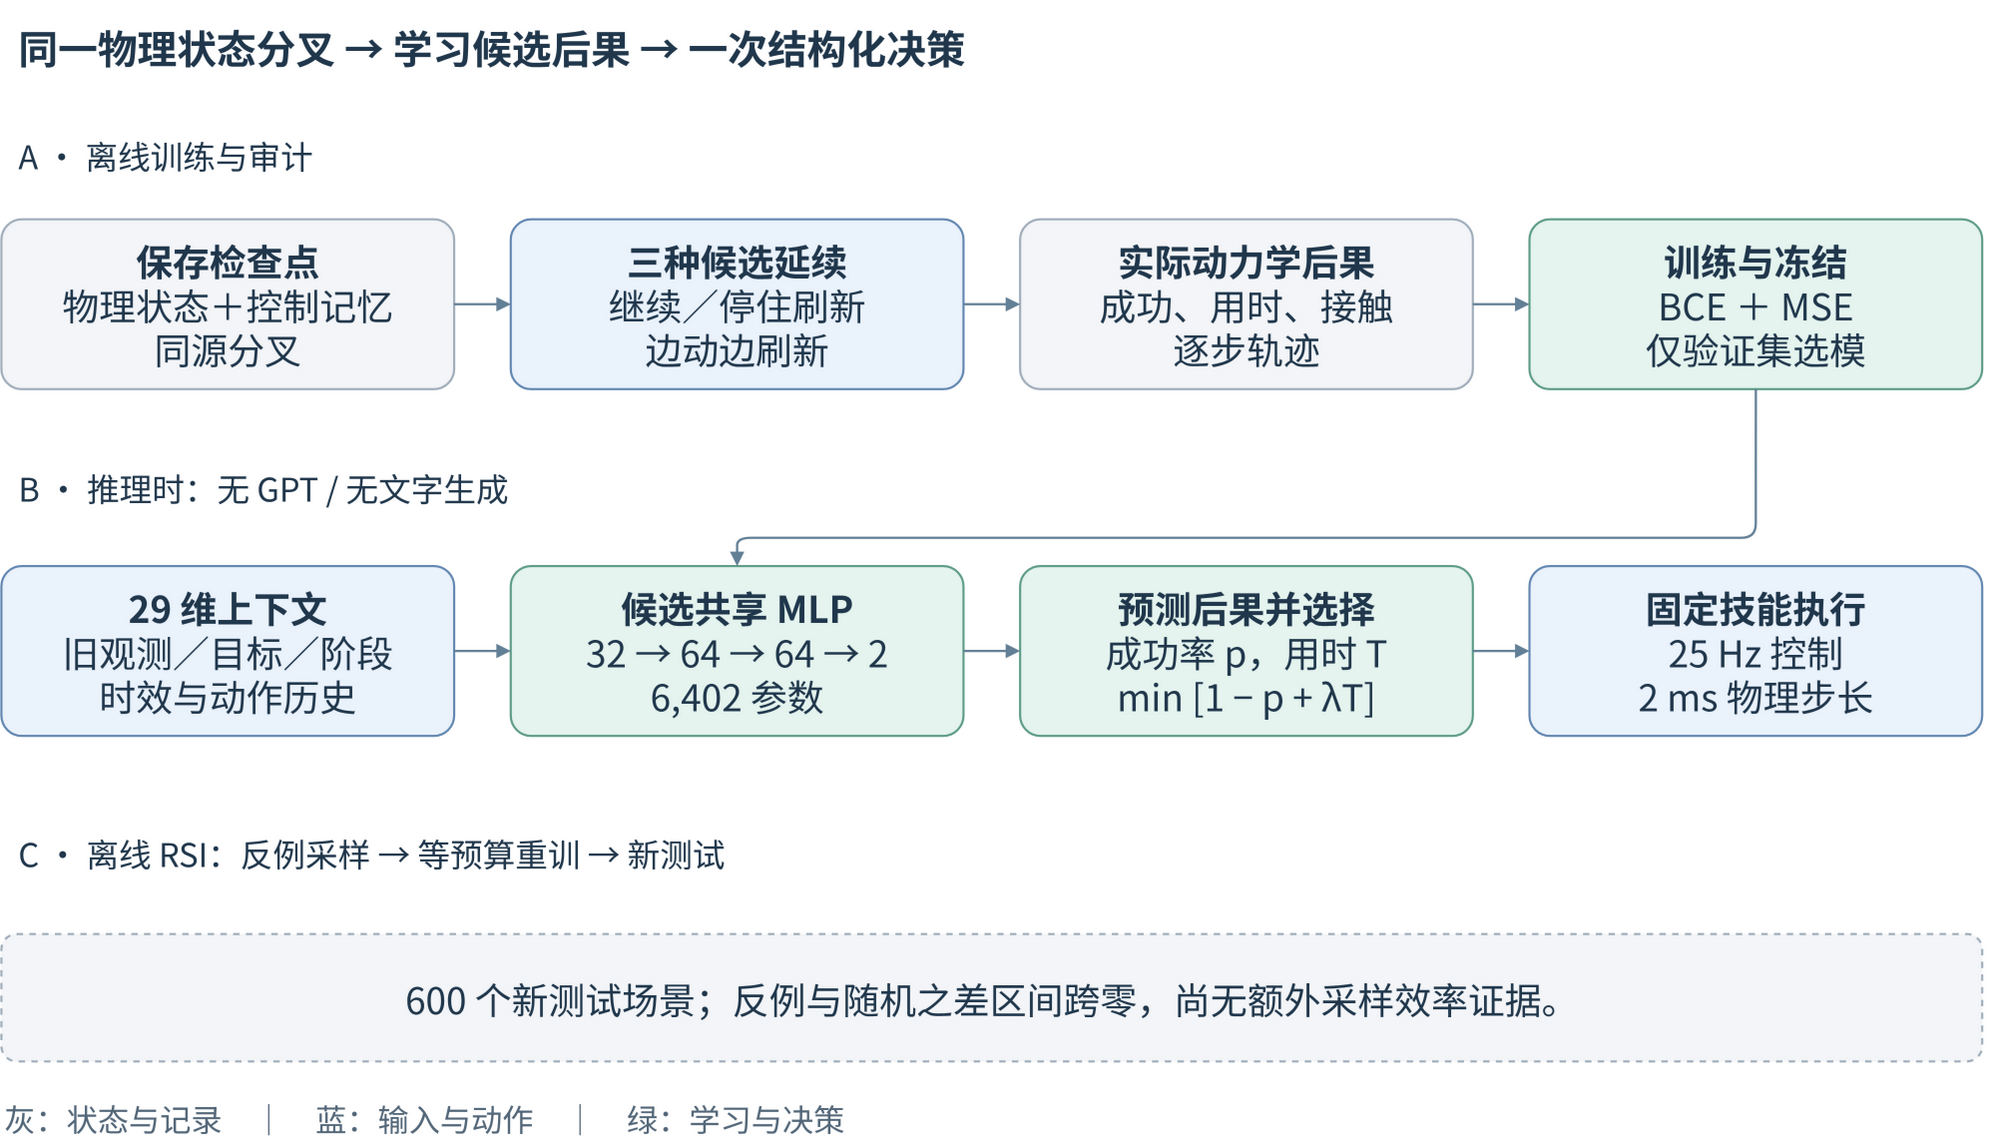
\includegraphics[width=\linewidth]{phase_pipeline.png}
\caption{实际实现的三个部分：配对分叉训练、有限候选判断、离线 RSI 更新。RSI 已完成一轮等预算检验，但未证实反例采样优于随机补数据。}
\label{fig:pipeline}
\end{figure}

\section{实验协议}
\paragraph{环境与控制器。}
使用 MuJoCo 3.6.0、Gymnasium 1.3.0、Gymnasium-Robotics 1.4.1 的 FetchPush-v4 和 FetchPickAndPlace-v4~\citep{plappert2018fetch,farama2026fetch}。
物理步长为 2 ms，控制周期为 40 ms。当前仿真使用 Fetch Cartesian 控制，不能视为双臂 Piper 或 200 Hz 真机链路的验证。
固定推物技能含背侧接近、下降和持续推动；推偏后抬升重定位，并限制接近点避免明显不可达目标。
抓取技能包括接近、下降、闭爪、抬升和搬运。
独立资格测试 seed 3000--3049 中，推物终局与最后十步保持均为 44/50，抓取均为 50/50。
推物低层失败是实验上限，本文不将全部失败归因于判断器。

\paragraph{检查点与分叉。}
前缀由精确物体观测驱动，按预先指定阶段和额外 0--5 步生成检查点。
未达到指定阶段的样本保留并标记；训练、验证、IID、长延迟集合分别有 7、2、6、1 个此类样本。
每个候选恢复完整 MjData、控制器记忆和传感器历史，并检查 integration state 一致。
所有分支具有相同的 150 个剩余控制步预算，评价要求连续 10 步满足环境的标准成功阈值。
总成本为 $C=1-y+\lambda T$，前缀用时不计入 $T$。
这一实验是干净前缀条件下的局部延续测试，而非从任务 reset 开始的端到端学习策略测试。

\paragraph{数据与冻结。}
训练 600、验证 180、IID 测试 360、长延迟测试 360 个检查点，每组两个任务均分，共 4,500 次候选执行。
样本年龄设定范围为 0--15 控制步，实际年龄由可用历史截断；训练及 IID 刷新延迟为 2--20 步，长延迟测试为 21--35 步。
噪声幅度均匀采样于 1--40 mm，时间价格为 0.02--0.15。
划分使用不同 reset seed 范围；网络种子为 11、22、33；它们是独立重复训练，推理时不作模型集成。
Adam 学习率为 0.002，全批训练 400 epoch，每 10 epoch 计算验证成本。
保存 checkpoint 哈希与所有基线规则后，才生成两组测试场景。

\paragraph{对照与统计。}
对照包括三个固定候选、验证集最优固定方式、按任务阶段查表以及验证集调优的年龄/噪声阈值规则。
完整模型与去阶段、去年龄、去历史三个变体使用相同网络，屏蔽标准化后的相应输入，共训练 12 个模型。
剩余特征可能透露被屏蔽变量的信息，因此这是特征移除消融，不是对阶段或历史的纯因果干预。
配对差值先在同一场景内平均三个网络种子，再按每任务 180 个场景 bootstrap 4,000 次。
报告的是探索性 95\% 区间，未作多重比较校正，也未覆盖训练种子总体的不确定性。

\section{结果与分析}
\begin{table}[t]
\centering\small
\caption{同分布留出测试。每个任务 180 个独立场景；网络方法为三个训练种子的均值。成功率越高越好，代价越低越好。}\label{tab:test}
\begin{tabular}{lrrrr}\toprule
方法 & Push 成功率 & Push 代价 & Pick 成功率 & Pick 代价\\\midrule
继续 & 57.8\% & 0.7475 & 86.1\% & 0.3558\\
停住刷新 & 84.4\% & 0.4277 & 100.0\% & 0.2144\\
异步刷新 & 85.6\% & 0.4109 & 98.3\% & 0.2081\\
阶段查表 & 84.4\% & 0.4285 & 100.0\% & 0.1918\\
完整判断器 & 85.4\% & 0.4071 & 99.1\% & 0.2034\\
去阶段 & 85.9\% & 0.4058 & 98.7\% & 0.2060\\
去年龄 & 85.2\% & 0.4086 & 98.3\% & 0.2115\\
去历史 & 86.9\% & 0.3925 & 98.7\% & 0.2062\\
\bottomrule\end{tabular}
\end{table}
\begin{table}[t]
\centering\small
\caption{长延迟留出测试。每个任务 180 个独立场景；网络方法为三个训练种子的均值。成功率越高越好，代价越低越好。}\label{tab:delay}
\begin{tabular}{lrrrr}\toprule
方法 & Push 成功率 & Push 代价 & Pick 成功率 & Pick 代价\\\midrule
继续 & 62.8\% & 0.6822 & 88.9\% & 0.3325\\
停住刷新 & 62.8\% & 0.7350 & 99.4\% & 0.2850\\
异步刷新 & 69.4\% & 0.6246 & 91.1\% & 0.3085\\
阶段查表 & 66.7\% & 0.6615 & 95.0\% & 0.2746\\
完整判断器 & 69.6\% & 0.6190 & 97.4\% & 0.2471\\
去阶段 & 68.3\% & 0.6425 & 95.4\% & 0.2639\\
去年龄 & 69.4\% & 0.6222 & 97.0\% & 0.2492\\
去历史 & 69.6\% & 0.6212 & 96.9\% & 0.2534\\
\bottomrule\end{tabular}
\end{table}

\paragraph{学习判断器并非全面胜出。}
同分布推物中完整模型平均成本约 0.4071，固定异步刷新约 0.4109，配对差值为 $-0.00383$，区间 $[-0.03197,0.02176]$。
同分布抓取中，完整模型减阶段查表的成本差为 $+0.01155$，区间 $[0.00124,0.02476]$。
这说明优于不刷新不足以建立贡献，简单的任务阶段先验已能解释相当部分收益。

\paragraph{长延迟抓取存在值得复核的局部信号。}
完整判断器平均成功率为 97.4\%，固定异步为 91.1\%，阶段查表为 95.0\%。
与固定异步的平均成本差为 $-0.06138$，区间 $[-0.09981,-0.02650]$；与阶段查表为 $-0.02747$，区间 $[-0.05938,-0.00049]$。
后一区间接近零，且本研究进行了多个探索性比较，不宜据此宣称稳定的普遍优势。
长延迟推物与固定异步的差值区间仍覆盖零。

\paragraph{阶段信号比动作历史更值得优先验证。}
长延迟抓取中，完整模型减去阶段变体的成本差为 $-0.01675$，区间 $[-0.03713,-0.00057]$。
但去年龄或去历史的区间覆盖零，其他条件下也没有一致优势。
当前结果不支持“加入动作历史即可得到更好的证据有效期模型”；下一轮应检验更明确的接触变化与感知遮挡，而不是扩大同类 MLP 后宣称解决了问题。

\begin{figure}[t]
\centering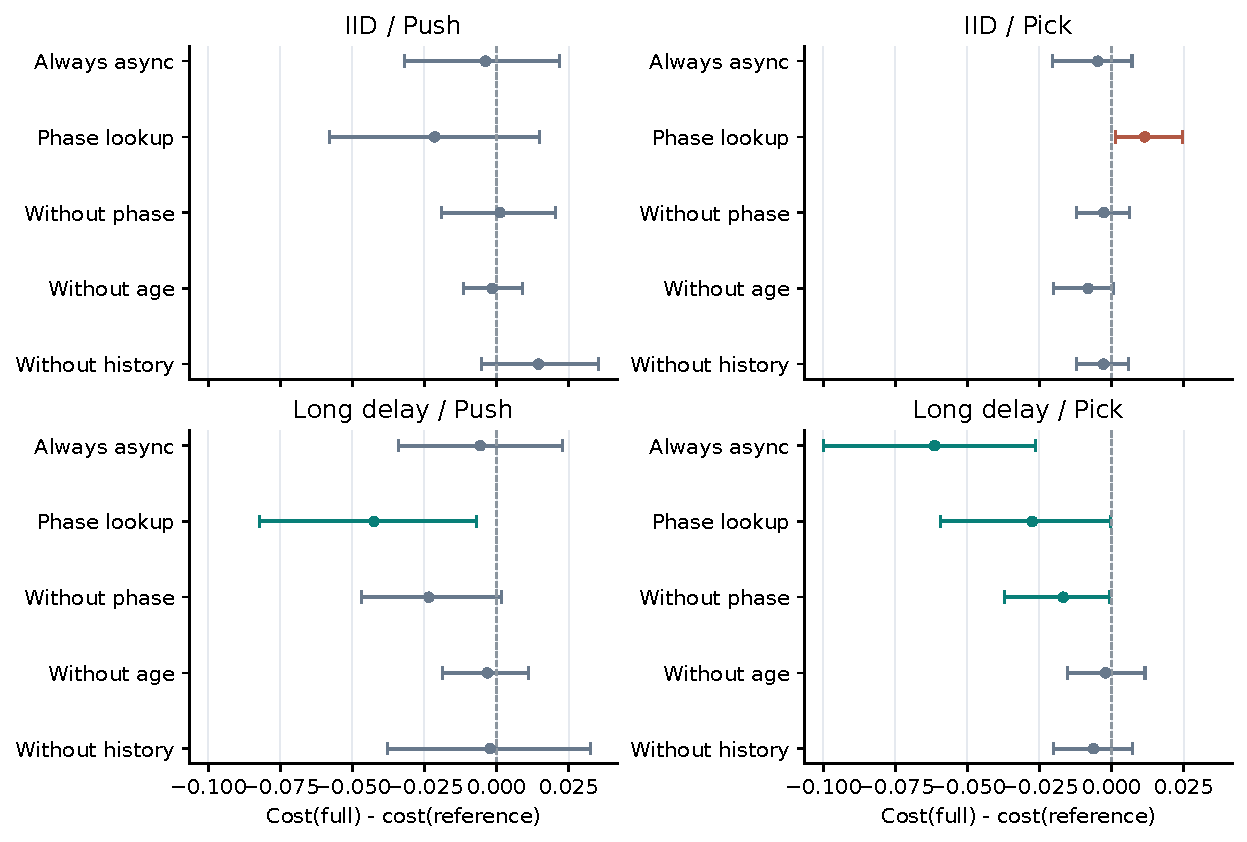
\includegraphics[width=\linewidth]{paired_effects.pdf}
\caption{完整模型相对强基线与消融的配对成本差。左侧为完整模型更好；灰色区间跨越零。每个子图有 180 个独立场景，区间为未作多重校正的探索性结果。}
\end{figure}

\paragraph{可复现性与过程证据。}
全部 4,500 条分支记录通过状态哈希、动作范围、时间序列、稳定成功和成本重算审计。
按固定索引选择的 10 个场景各录制三个候选，共 30 段视频。
渲染前后保存并恢复 MjData，30 段录像的逐步记录与无渲染评测完全一致。
这种检查解决了渲染影响内部求解状态的问题，但不证明跨硬件或跨 MuJoCo 版本的逐位一致。

\section{RSI：一轮等预算数据更新检验}
我们进一步完成训练侧反例采样、物理采集、模型更新和新测试集验证的一轮离线闭环。
复用原 600 个训练场景，以按任务和阶段分层的三折交叉拟合、三个模型种子估计决策遗憾
$r_i=C_i(\hat a_i)-\min_a C_i(a)$；不读取旧测试标签。
在 1,200 个只有可见输入、尚无候选结果标签的检查点中，以同任务 15 个标准化近邻的加权遗憾评分。
这是一种常规反例导向采样原型，不主张近邻回归或主动学习本身具有新颖性。

随机、模型分歧、反例导向三种策略各获得 180 个场景、540 条候选执行预算。
各任务与延迟区间均衡；两种定向方法均保留 20\% 随机探索。
请求合并后实际有 393 个不同场景。三个采样策略和仅重训旧数据的控制组都从同一原模型初始化，
固定归一化、400 次 Adam 更新、每次 256 个场景，使用新的 180 个验证场景选择 checkpoint，允许保留第 0 步原模型。
冻结权重后，才构建两个各 300 场景的新测试集，共 600 个独立场景；网络种子仍为 11、22、33。更新集已含长延迟，因此新长延迟集合属于目标域的新场景留出，不再是更新模型未见的延迟分布。

\begin{table}[t]
\centering\small
\caption{离线 RSI 更新后的新测试成本；学习模型取三个种子均值，固定策略共用同一组场景。每组 300 场景，各任务 150 个。}
\begin{tabular}{lrr}\toprule
方法 & 新 IID & 新长延迟 \\\midrule
冻结原模型 & 0.31673 & 0.42037 \\
只重训旧数据 & 0.31772 & 0.41974 \\
随机补数据 & 0.31499 & 0.40678 \\
模型分歧补数据 & 0.32076 & 0.40840 \\
反例补数据 & 0.31005 & 0.40247 \\
固定异步刷新 & 0.30952 & 0.43032 \\
任务阶段查表 & 0.30407 & 0.42655 \\\bottomrule
\end{tabular}
\end{table}

预先指定的主要对照为两个分布等权合并后的反例减随机成本差：$-0.00462$，
按 600 个场景 bootstrap 的 95\% 区间为 $[-0.01409,0.00439]$。
相对模型分歧的差为 $-0.00832$，探索性区间 $[-0.01839,0.00144]$。
二者均跨零，尚不能支持反例采样具有额外样本效率。
相对冻结模型或只重训旧数据的改善不能替代等新增数据预算的比较。新 IID 中阶段查表成本仍低于反例更新模型，不能主张全面优于强规则。
本轮只有一次采样随机实现，区间不覆盖采样种子总体；不能将一次更新解释为持续自我改进。

\paragraph{计算资源与可移植性。}
IDC 的八个 CPU worker 完成候选前缀、验证、补数据和两个测试集的采集，分别耗时约
7.1、15.1、29.5、20.2、22.8 秒；含 12 个跨机器预检场景的 3,555 条候选分支均通过审计。
模型交叉拟合和更新在另一台开发机上完成，未提交集群训练任务。
归档的 GPU 环境使用 PyTorch 2.7.1+cu128、\texttt{high} 浮点矩阵精度及 TF32，分数不要求与 CPU 逐位相等。
固定导出的反例模型 seed 11 在 NumPy CPU 上与原记录的 600 个候选选择全部一致；
单场景三候选判断的中位耗时为 0.054 ms，P99 为 0.065 ms（100 次预热、2,000 次计时，单 BLAS 线程）。
该测量仅覆盖驻留判断头及归一化/评分，不含视觉、通信、IK 或伺服，不能据此宣称完整机器人链路达到相同频率。
新增录像直接播放归档 qpos/qvel。Fetch 抓取环境的派生位姿缓存与积分状态相差一个 2 ms 物理步；位姿核对按原生观测时刻对齐，视频显示保存的积分状态~\citep{mujoco2026simulation}。
一个跨机器重跑案例出现约 $10^{-13}$ 的速度差，其成功、用时和成本相同；本文不要求跨机器逐位一致。

\section{局限与论文成熟度}
第一，当前只有两个接触任务，且使用已知任务标签和手写技能，没有任务语义学习、自由候选生成或跨构型迁移。
第二，Gymnasium 本体观测（无附加噪声）与合成带噪物体位置不等同于真实视觉系统；干净前缀会低估闭环累积错误。
第三，每个检查点只有一次判断，尚未研究持续重规划、取消在途请求或推理请求队列。
第四，候选真实结果在仿真中可配对，并不意味着真机可同成本获取这些标签。
第五，模型概率未经独立校准，训练规模有限，统计比较尚需预注册确认性复验。

当前工作量足以形成一份可复现的内部研究稿，并可作为 workshop 短稿的起点；仍不足以支撑普遍优越性、持续在线机器人自改进或顶会主会级创新主张。
主会方向需要增加至少一种不同接触机制、真实图像观测、全任务连续闭环，以及等预算强方法比较。
已有 Piper 历史抓取成功记录仅作为系统背景，不作为本学习判断器的真机实验。

\section{结论}
配对物理仿真使机器人信息决策的收益与代价可被直接审计。
小型非生成式判断器在长延迟抓取上表现出局部潜力，但强规则与消融限制了更强的解释。
一轮离线 RSI 更新未证明反例选择优于等预算随机采样。下一步应优先构造能区分机制的执行队列与接触变化实验，再在新任务、真实视觉和多个采样种子上验证。

\bibliography{references}
\end{document}
